
\chapter{引言}%

% \newcommand\clearpageT{\clearpage}
% \newcommand\cleardoublepageT{\cleardoublepage}
% \renewcommand{\clearpage}{}
% \renewcommand{\cleardoublepage}{}
随着数字技术的快速发展,数字信号处理已深入到各个学科领域。在数
字信号处理中,许多算法如相关、滤波、谱估计、卷积等都可通过转化为
离散傅立叶变换(DFT)实现,从而为离散信号分析从理论上提供了变换工具。但
    DFT计算量大,实现困难。快速傅立叶(FFT)\cite{fft} 的提出,大大减少了计算量,从根
本上改变了傅立叶变换的地位,成为数字信号处理中的核心技术之一,广泛应用
于雷达、观测、跟踪、高速图像处理、保密无线通信和数字通信等领域。

目前,硬件实现FFT算法的方案主要有:通用数字信号处理器(DSP)、FFT
专用器件和现场可编程门阵列(FPGA)。DSP具有纯软件实现的灵活性,适用
于流程复杂的算法,如通信系统中信道的编译码、QAM映射等算法。
DSP完成FFT运算需占用大量DSP的运算时间,使整个系统的数据吞吐率降低,
同时也无法发挥DSP软件实现的灵活性。采用FFT专用器件,速度虽能够达到
要求。但其外围电路复杂,可扩展性差,成本昂贵。随着FPGA发展,其资源
丰富,易于组织流水和并行结构,将FFT实时性要求与FPGA器件设计的灵活性
相结合,实现并行算法与硬件结构的优化配置,不仅可以提高处理速度,并且
具有灵活性高。开发费用低、开发周期短、升级简单的特点。
本文进行了DIT-FFT的Verilog实现,并以16位长数据,16点FFT为例,
用modelsim仿真,软件上通过综合和仿真。

\chapter{FFT原理概述}

FFT算法就是不断地把长序列的DFT分解成几个短序列的DFT,并利用旋转因子
$W_N^{kn}$ 的周期性和对称性来减少DFT的运算次数\cite{dsp} 。最简单最常用的
是基2FFT,其算法分为两类:DIT-FFT和DIF-FFT,本文采用的是第一种。

\section{DIT-FFT基本原理}

设序列$x(n)$的长度为 $N$,且满足 $N=2^M$,$M$ 为自然数。按$n$ 的奇
偶把$x(n)$ 分解为两个$N /2$的子序列。
 \begin{equation*}
    \begin{aligned}
        x_1(r)&=x(2r)& \quad &r=0,1,\dots,\frac{N}{2}-1\\
        x_2(r)&=x(2r+1)& &r=0,1,\dots,\frac{N}{2}-1
    \end{aligned}
\end{equation*}
则$x(n)$ 的DFT为

\begin{equation}
    \begin{aligned}
    \label{eq:1}
        X(k)&= \sum_{n~is~even} x(n)W_N^{kn}+\sum_{n~is~odd}x(n)W_N^{kn}\\
            &= \sum_{r=0}^{N /2 -1}x(2r)W_N^{2kr}+\sum_{r=0}^{N /2-1} x(2r+1)W_{N}^{k(2r+1)}\\
            &= \sum_{r=0}^{N/2-1}x_1(r)W_N^{2kr}+W_N^k\sum_{r=0}^{N/2-1}x_2(r)W_N^{2kr}\\
            &= \sum_{r=0}^{N/2-1}x_1(r)W_{N /2}^{kr}+W_N^k\sum_{r=0}^{N/2-1}x_2(r)W_{N /2}^{kr}\quad (W_N^{2kr}=W_{N/2}^{kr})\\
            &=X_1(k)+W_{N}^kX_2(k)\quad k=0,1,2,\dots,N-1
    \end{aligned}
\end{equation}
其中$X_1(k)$ 和$X_2(k)$ 分别为$x_1(r)$ 和$x_2(r)$ 的$N /2$点DFT,即:
\begin{equation}\label{eq:3}
     X_1(k)=\sum_{r=0}^{N /2-1} x_1(r)W_{N/2}^{kr}=DFT[x_1(r)]_{N /2}
\end{equation}

\begin{equation}\label{eq:4}
     X_2(k)=\sum_{r=0}^{N /2-1} x_2(r)W_{N/2}^{kr}=DFT[x_2(r)]_{N /2}
\end{equation}
由于$X_1(k)$ 和$X_2(k)$ 均以$N /2$为周期,并且 $W_N^{k+ N /2}=-W_N^k$,因此 $X(k)$ 又
可以表示为:

\begin{equation}
    \begin{aligned}
        \label{eq:5}
        X(k)&=X_1(k)+W_N^kX_2(k)&\quad & k=0,1,\dots,\frac{N}{2}-1\\
        X(k+\frac{N}{2})&=X_1(k)-W_N^kX_2(k)&\quad & k=0,1,\dots,\frac{N}{2}-1
    \end{aligned}
\end{equation}
这样,就将$N$ 点DFT分解为两个$N /2$点DFT和\ref{eq:5} 式的运算,\ref{eq:5}式的运算
可以由图\ref{fig:buttery}的流图符号表示,称为蝶形符号。
\begin{figure}[htpb]
        \centering
            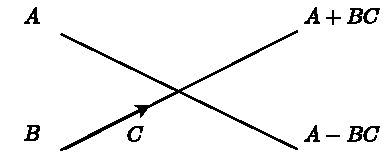
\includegraphics[width=0.4\linewidth]{Figure/butteryfly.pdf}
\caption{蝶形运算符号}%
\label{fig:buttery}
\end{figure}

    由图 \ref{fig:buttery}可以看出,完成一个蝶形运算,需要一个复数乘法和两次复数加法运算。

$N=2^M$, $N/2$ 仍然是偶数,故可以对 $N /2$点DFT再进行进一步分解。
与第一次分解相同,将 $x_1(r)$按照奇偶分解为 $\frac{N}{4}$ 点的子序列。

……

经过 $M$轮分解,最后得到 $N$ 点DFT分解成 $N$ 个DFT和 $M$ 级蝶形算符,而1点
DFT就是时间序列本身。图中输入序列不是顺序序列,但后面可以看到,其排列是有
规律的。
\begin{figure}[H]
    \centering
        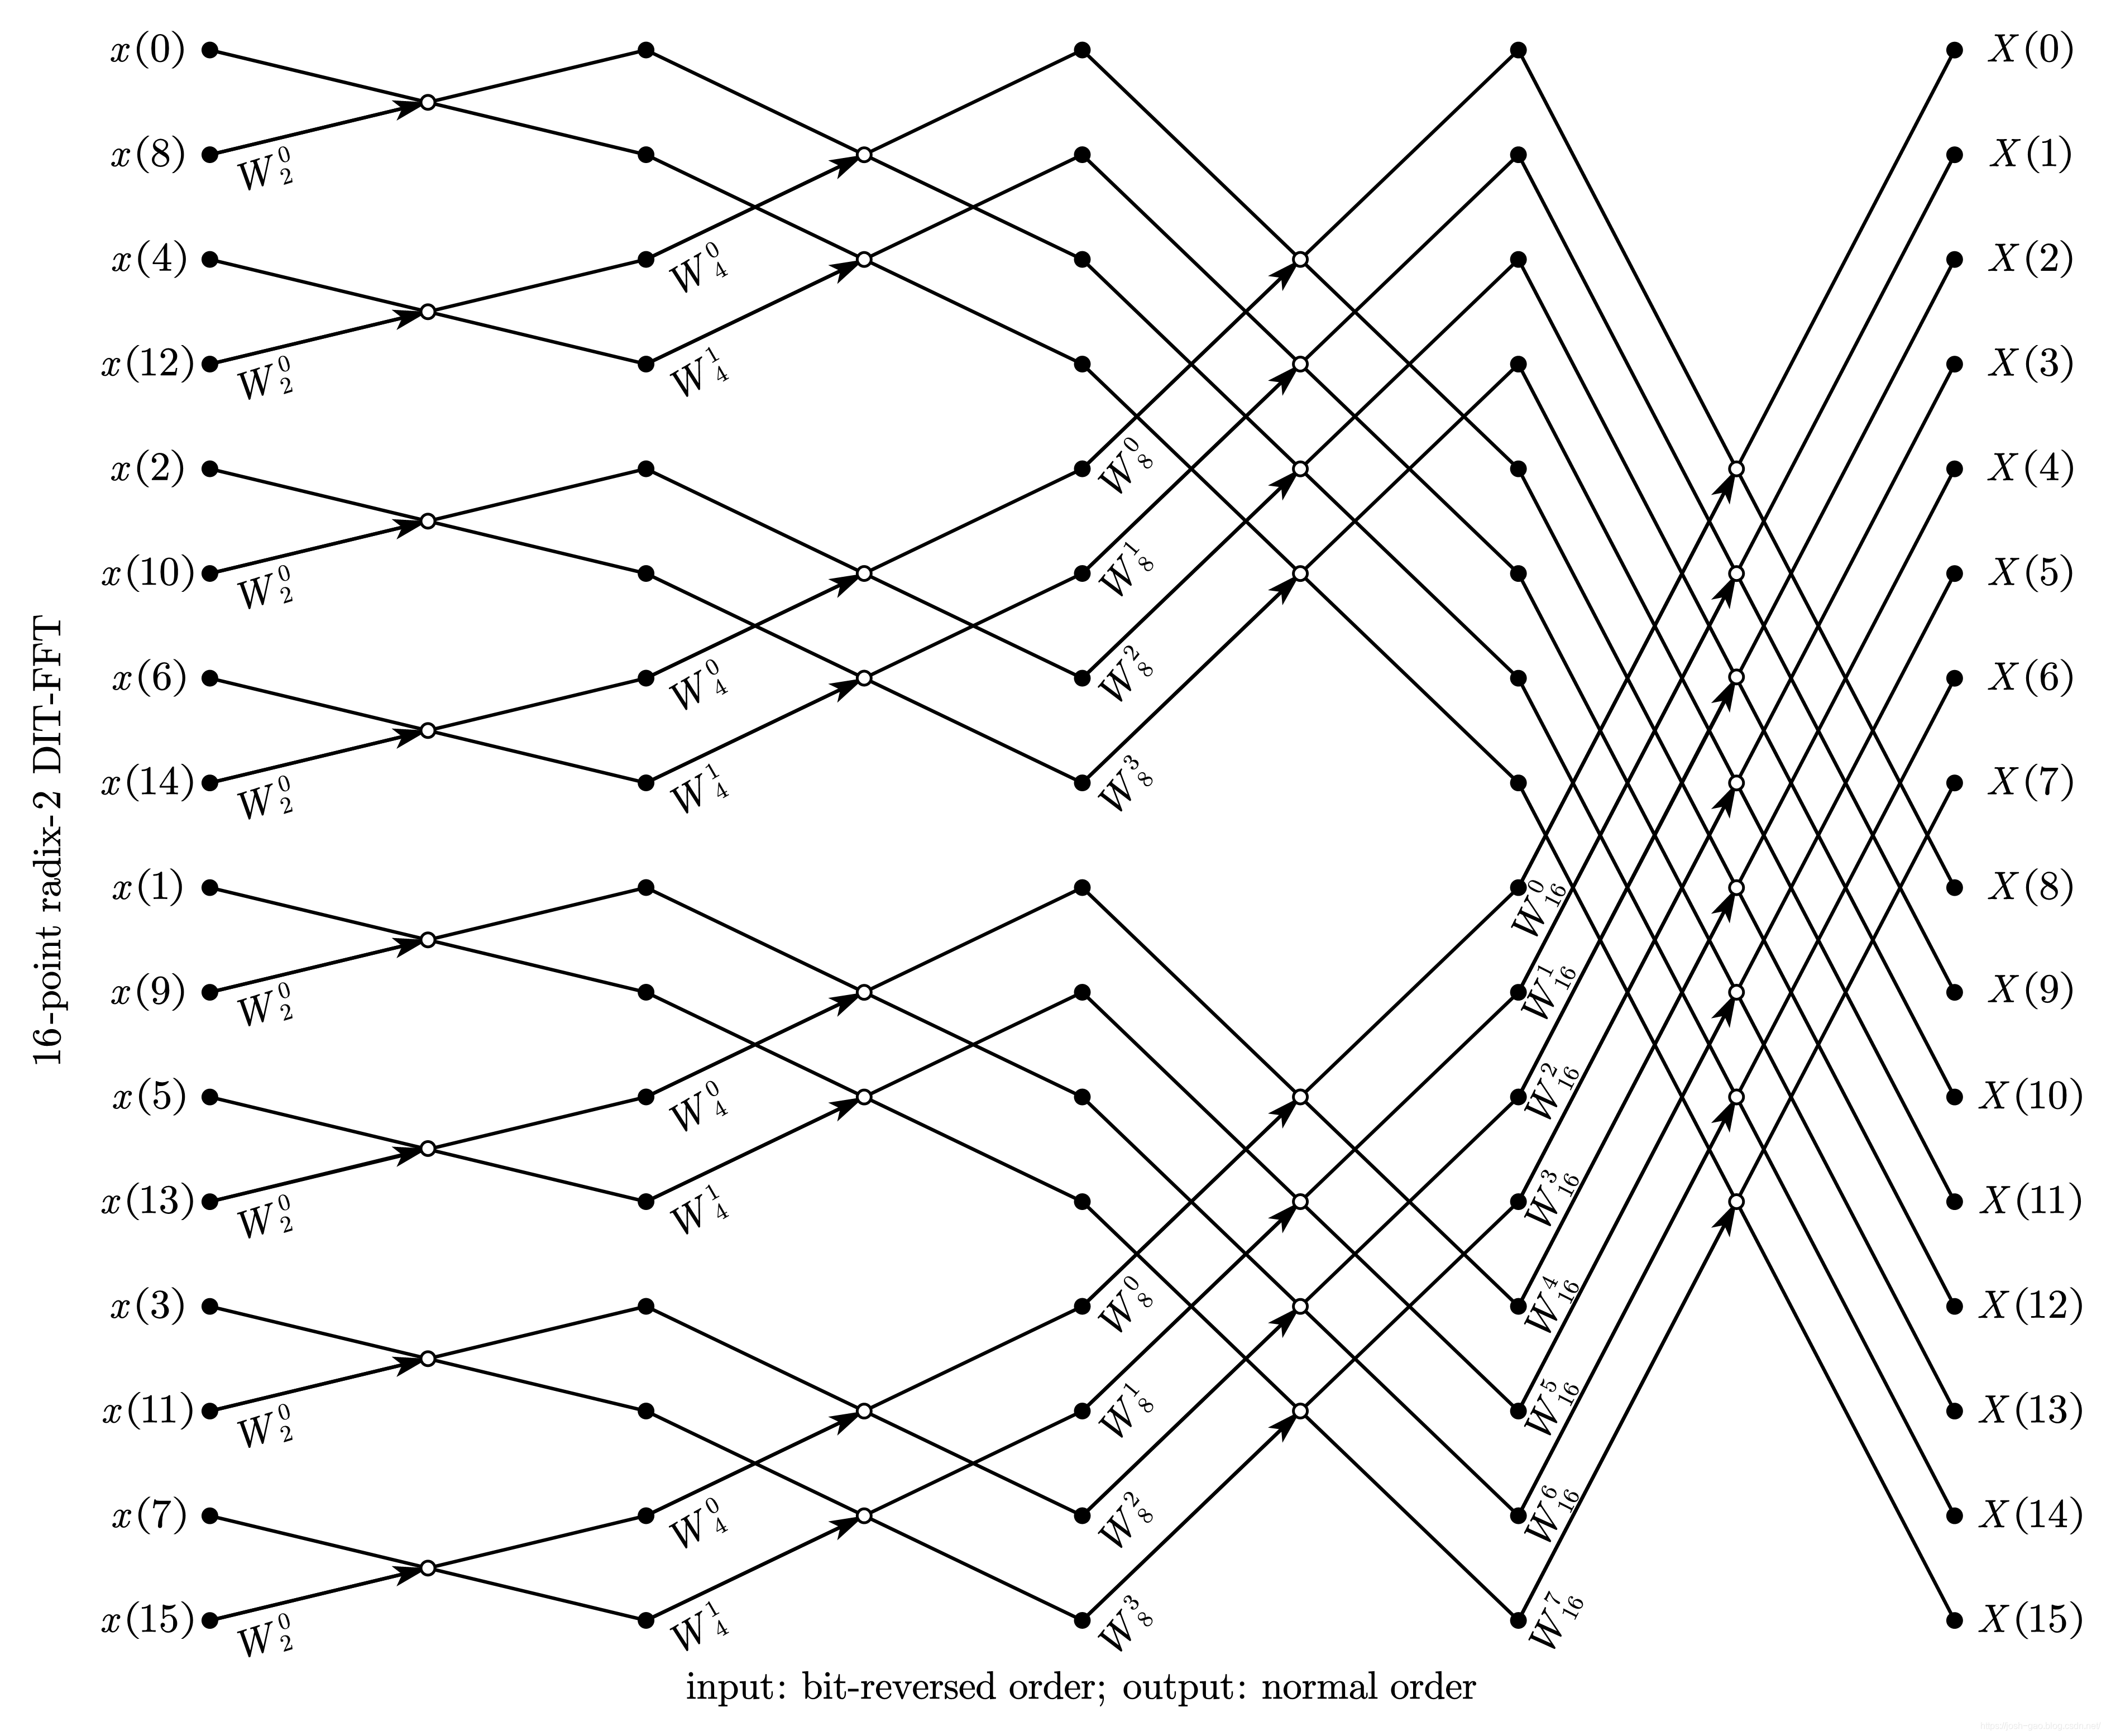
\includegraphics[width=0.8\linewidth]{Figure/dataflow.png}
    \caption{16点DIT-FFT的运算流图}%
    \label{fig:Figure/dataflow}
\end{figure}

\section{运算规律和编程思想}%


为了方便设计出DIF-FFT的硬件电路,下面介绍DIF-FFT的运算规律和编程思想。

\subsection{原位计算}%
\label{sub:yuan_wei_ji_suan_}



由图\ref{fig:Figure/dataflow},可以看出。 $N=2^M$ 点的FFT共进行 $M$ 级运算,每级由
$N /2$ 个蝶形组成。计算完一个蝶形后,所得的输出数据可以立即存入原输入数据所占用的
存储单元(数组元素)。这样,经过 $M$级运算后,原来存放输入序列的 $N$ 个存储单元便依次
存放 $X(k)$ 的 $N$ 个值。因为 $M$ 级,存储单元的值要每一级进行更新,所以需设计 \textbf{$N$ 个RAM单元}。
这种利用同一存储单元存储蝶形计算输入、输出数据的方法称为原位计算。原位计算可以节省大量内存,
从而使设备成本降低。
\label{ssub:yuan_wei_ji_suan_}

\subsection{旋转因子的变化规律}%
\label{sub:xuan_zhuan_yin_zi_de_bian_hua_gui_lu_}

每个蝶形都要乘一个因子 $W_N^p$,称为旋转因子, $p$ 为旋转因子的指数。(在Verilog中,可以用一个\textbf{ROM}来存储旋转因子的数值)但各级的旋转因子和循环
方式都有所不同。应获得旋转因子 $W_N^p$ 与运算级数的关系。用 $L$ 表示从左到右的运算级数 $L=1,2,\dots,M$.
观察图\ref{fig:Figure/dataflow}可以发现,第$L$ 级共有$2^{L-1}$ 个不同的旋转因子。第$L$ 级的旋转因子
为

\begin{equation}\label{eq:calJ}
    W_N^p=W_{2^L}^J=W_{N\cdot 2^{L-M}}^J=W_N^{J\cdot 2^{M-L}} \quad J=0,1,2,\dots,2^{L-1}-1
\end{equation}
这样,就可以通过\ref{eq:calJ}式来确定第$L$ 级的旋转因子。

\subsection{蝶形运算规律}%
\label{sub:die_xing_yun_suan_gui_lu_}

设序列$x(n)$ 经时域抽选(倒序)后,按照图\ref{fig:Figure/dataflow}存入数组(内存)$A$中。如果蝶形
运算的两个输入数据相互距离 $B$ 个点,应用原位计算,有

\begin{equation*}
    \begin{aligned}
        A_L(J)&\Leftarrow A_{L-1}(J)+A_{L-1}(J+B)W_N^p\\
        A_L(J+B)&\Leftarrow A_{L-1}(J)-A_{L-1}(J+B)W_N^p
    \end{aligned}
\end{equation*}
式中$p=J\times 2^{M-L}\quad J=0,1,\dots,2^{L-1}-1;L=1,2,\dots,M$

\subsection{编程思想及程序框图}%
\label{sub:bian_cheng_si_xiang_}

\tikzstyle{startstop} = [rectangle, rounded corners, minimum width = 2cm, minimum height=1cm,text centered, draw = black]
\tikzstyle{io} = [trapezium, trapezium left angle=70, trapezium right angle=110, minimum width=2cm, minimum height=1cm, text centered, draw=black]
\begin{figure}[H]
    \centering
    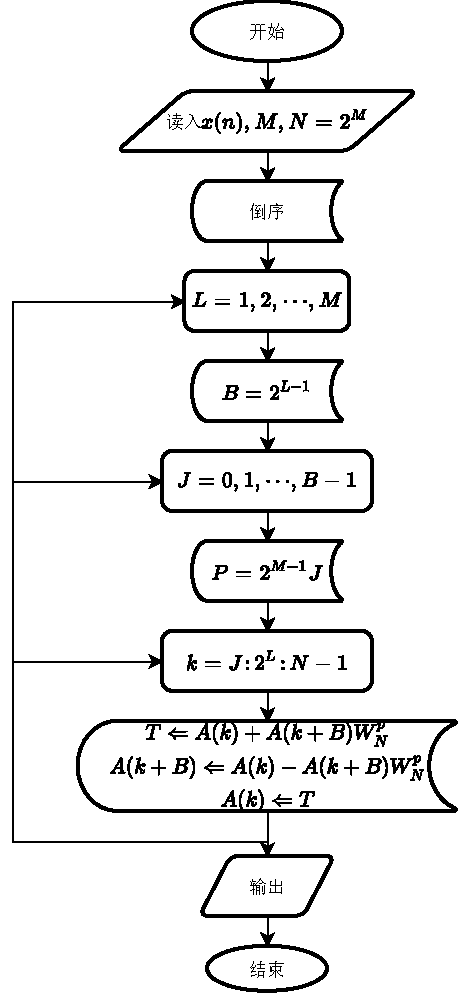
\includegraphics[scale=0.618]{Figure/flowchat.pdf}
    \caption{DIT-FFT运算程序图}%
    \label{fig:flowchat}
\end{figure}


\subsection{序列的倒序}%
\label{sub:xu_lie_de_dao_xu_}

DIT-FFT算法运算流图的输出$X(k)$ 为自然顺序,但为了适应原为计算,其输入序列不是按照$x(n)$ 的
自然顺序排列,这种经过$M$ 次偶奇抽选后的排序称为序列$x(n)$ 的倒序(0-N-1十进制数转为二进制数,然后翻转二进制数,译出十进制数)
。因此,在运算$M$ 级蝶形之前应先对序列$x(n)$ 进行倒序。

\section{定点数与有限字长效应}


定点数指的是在二进制数中小数点的位置是固定的数,在本设计中采用定点数,目的是
浮点运算在Verilog中耗时较慢。浮点数虽然扩大了数的表示范围,但这是以降低精度为代价。
浮点运算要比定点运算复杂,定点运算时,当运算结果超出数的表示范围,就会发生溢出。


当FPGA实现乘法运算时,例如计算两个$N$ 位宽的二进制数的乘积,乘积的结果一半都会用
$2N$ 位宽的二进制数表示,此时都会将结果进行适当的舍位处理,以较少最终的数据宽度。
进行舍位就会引入误差,这种误差术语运算量化误差,也称为运算噪声。

\chapter{Verilog设计思路及说明}

\section{设计框图}
图\ref{fig:Figure/verilog-design}给出了FFT算法的结构框图。这种形式的FFT只有一个蝶形运算单元
,蝶形运算按照递归的方式,根据蝶形图从左往右,从上向下先计算第一级的每个蝶形,然后计算
第二级,第三级,逐级地进行运算,直至第$\frac{N}{2}\log_2 N$ 个蝶形,完成$N$ 点
FFT的全部计算。

在实际设计时,可以将输入缓冲单元和输出缓冲单元做成同一个存储单元。这种结构
的优点是只有一个蝶形运算单元,所占的硬件资源少,结构简单,稳定性能好,
    缺点是运算速度缓慢,且时序控制较为复杂\cite{github}。
\begin{figure}[H]
    \centering
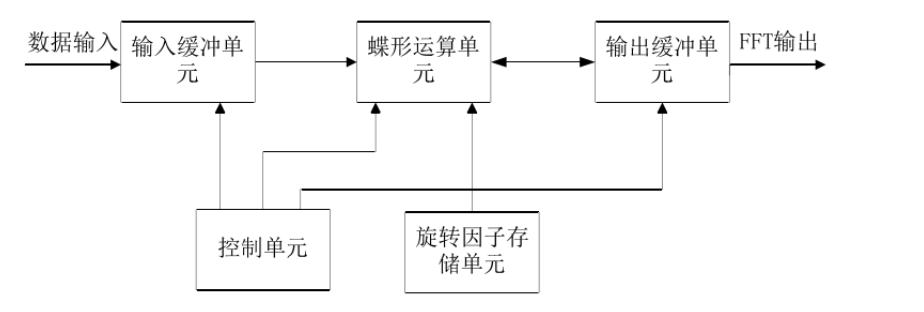
\includegraphics[width=0.8\linewidth]{Figure/verilog-design.png}
    \caption{Verilog设计结构框图}%
    \label{fig:Figure/verilog-design}
\end{figure}

\textbf{以下所有的单元设计对应的Verilog程序见 \url{https://github.com/DestinyEnvoy/Fast-Fourier-Transform/tree/master/unit/}}

\section{存储单元设计}

\subsection{缓冲单元(RAM)}
\textbf{{mem\_32x16.v}文件实现16个32bit的内存单元}。每一个单元前16bit存储复数的实数部分,后16bit存储复数的叙述部分 。
        通过内容\ref{ssub:yuan_wei_ji_suan_}可以知道,每个蝶形运算的输入、输出数据均要
        经过RAM的读写操作,因此RAM的频繁读写操作速度对FFT的处理速度影响较大。为了加快速度
        ,我们设计可以同时读取/写入两个单元数据的RAM,加速蝶形运算。
        \subsection{旋转因子存储单元(ROM)}

\textbf{w\_lut.v文件实现8个旋转因子的存储,即 $W_{16}^0,W_{16}^1,\dots,W_{16}^7$ }。每个旋转因子
用32bit存储,高16bit存储实数部分,低16bit存储虚数部分,每部分存储都用2.14格式的定位数存储。
即第 $k$个旋转因子实数,虚数部分分别存储 $2^{14}\cos{\frac{2k\pi}{16}}$,$-2^{14}\sin{\frac{2k\pi}{16}}$整数部分的二进制码。

\subsection{地址发生存储单元(ROM)}%
\label{sub:di_zhi_fa_sheng_cun_chu_dan_yuan_rom_}

\textbf{read\_addr\_lut.v文件实现了第 $L$级第  $k$个蝶形单元,
需要结合的三个数据  $X(k)$,  $X(k+B)$ , $W_N^p$的
在以上RAM,ROM对应的地址信息。}如第0级第0个蝶形结合RAM钟
第0第8个数据,第0个蝶形存储单元,这三个地址对应的数参与蝶形运算。(参照图\ref{fig:Figure/dataflow})
该地址发生存储单元是控制单元的一部分。

\section{蝶形运算单元}

\textbf{bufferfly.v文件实现了复数的蝶形运算},运算原理参考图\ref{fig:buttery}。蝶形运算两个端口输出也是32bit,
高实,低虚数,第一二三四级蝶形输出分别是9.7,10.6,11.5,12.4格式的定位数。同时对该蝶形运算做了饱和溢出与舍入处理:
高于最大正数32'h7fff0000 计做16'h7fff,小于最大负数32'h80000000,计为16'h8000,
否则取乘法结果的第28到13位作为数据输出。
\section{控制单元}

\textbf{fft\_ctrl\_sm.v文件实现每一个蝶形运算前后所有的控制信息}。如某个蝶形
运算接收后,下一个蝶形序号的变化或是否进入下一级FFT,以及此时RAM的读写控制信号。
很容易知道,该单元包含了地址发生单元(ROM)。

\textbf{fft\_top.v文件实现所有单元信号的综合}。是最顶层的模块。

\chapter{波形仿真及其分析}

\textbf{以下两个test bench 文件对应Verilog源码见 \url{https://github.com/DestinyEnvoy/Fast-Fourier-Transform/tree/master/sim}}

\section{蝶形运算单元}

\textbf{butterfly\_tb.v文件实现了蝶形运算单元的仿真}。蝶形运算单元是FFT设计中最重要的一部分,因此我们对蝶形运算单元进行分析。

我们设计一个test bench,使得输入一个8.8格式的数据输入 $A=2.5+5.25j$, $B=6+1.5j$, $C=1+0.375j$,
因此输出 $Y=A-BC=-2.9375+1.5j,X=A+BC=7.9375+9j$,  $X,Y$写成
9.7格式的定位数 $2^7Y=-376+192j,2^7X=1016+1152j$,详细计算如下表\ref{tab:value}

\begin{table}[H]
    \centering
    \caption{蝶形运算单元理论值}
    \label{tab:value}
    \begin{tabular}{|cccc|}
        \hline
        输入 & $A$ & $B$ & $C$\\ 
        浮点数 &  $2.5+5.25j$ &  $B=6+1.5j$ & $1+0.375j$ \\
        定位数(8.8 /2.14格式) & $640+1344j$ & $1536+384j$ & $16384+6114j$\\
        \hline
        输出 & $X=A+BC$ &  $Y=A-BC$ &  \\
        浮点数 & $7.9375+9j$ &  $-2.9375+1.5j$ &\\
        定位数(9.7格式) &  $1016+1152j$ &  $-376+192j$ &\\ \hline
    \end{tabular}
\end{table}
\begin{figure}[H]
    \centering
    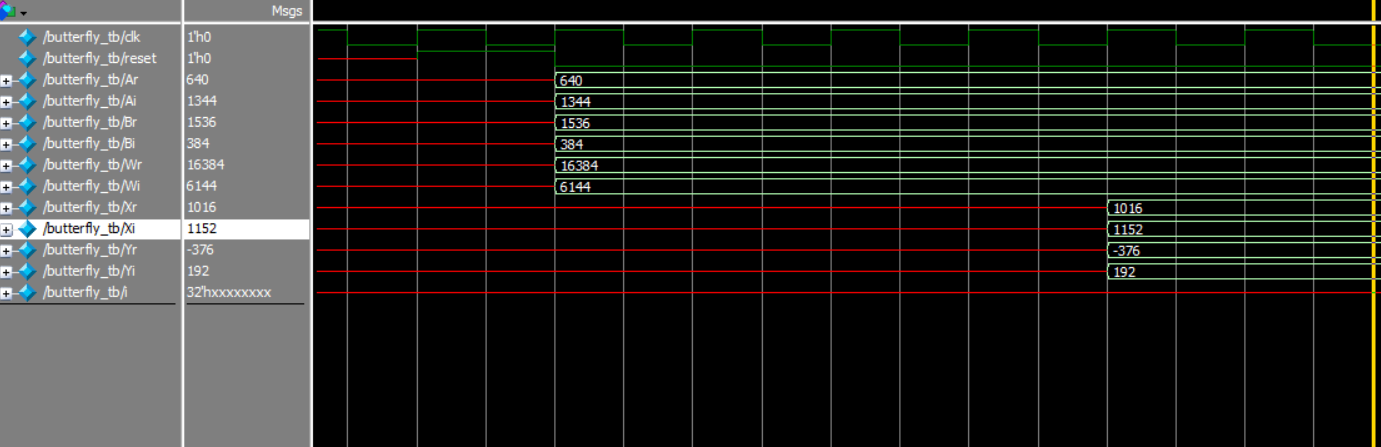
\includegraphics[width=0.9\linewidth]{Figure/buttery_sim.png}
    \caption{蝶形运算单元仿真}%
    \label{fig:but_sim}
\end{figure}
对比表\ref{tab:value}和图\ref{fig:but_sim},可以发现,两者结果相同,蝶形运算单元可以正常工作。

\section{FFT所有单元}

\subsection{Verilog仿真}
\textbf{fft\_top\_tb.v文件实现了fft单元的仿真测试。}我们分两路传输复数,第一路串行输入复数的实部,第二路同步串行输入复数的虚部。输入都是8.8格式的定位
数。
如下图:

\begin{figure}[H]
    \centering
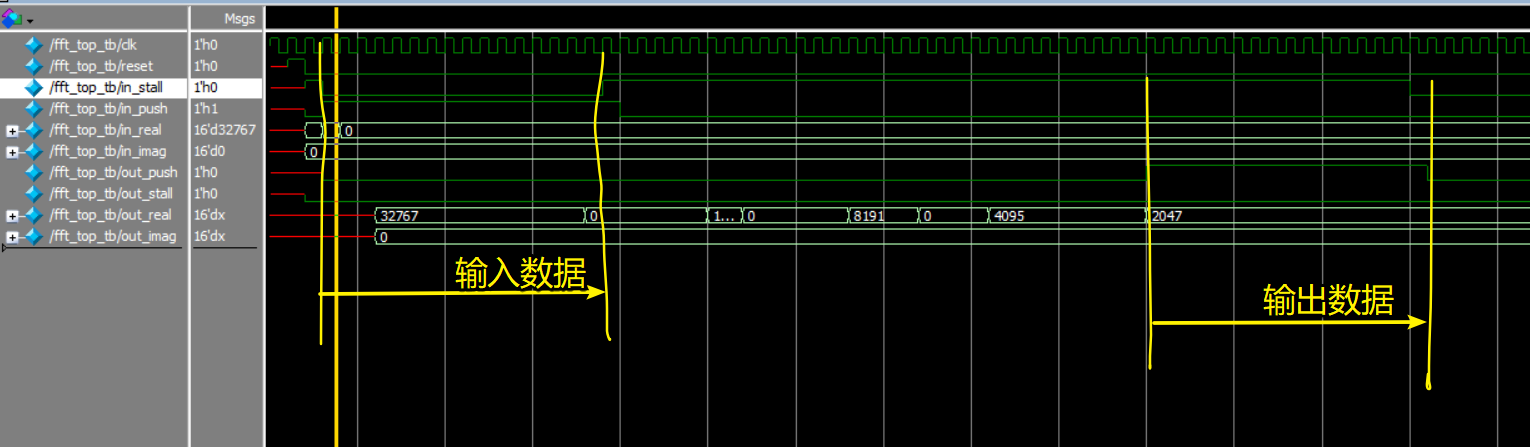
\includegraphics[width=\linewidth]{Figure/fft_sim.png}
    \caption{FFT单元仿真}%
    \label{fig:fft_sim}
\end{figure}
输入$x(0)=(2^{15}-1) /2^8,x(k)=0,k=\text{其他}$ ($x(0)$为Verilog输入的最大值),理论得出 $X(k)=x(0) /16$,其12.4格式
的定位数为 $\lfloor 2^4 X(k)\rfloor=2047$。图\ref{fig:fft_sim}与理论相符。

\subsection{与matlab仿真对比}
测试四组数据(fft\_top\_tb.v中有四组数据的生成方式),得到matlab的数据以及verilog FFT单元的
FFT(忽略了小数的舍入误差),如下图\ref{fig:duibi}


\begin{figure}[H]

    \begin{center}
            \subcaptionbox{数据1}{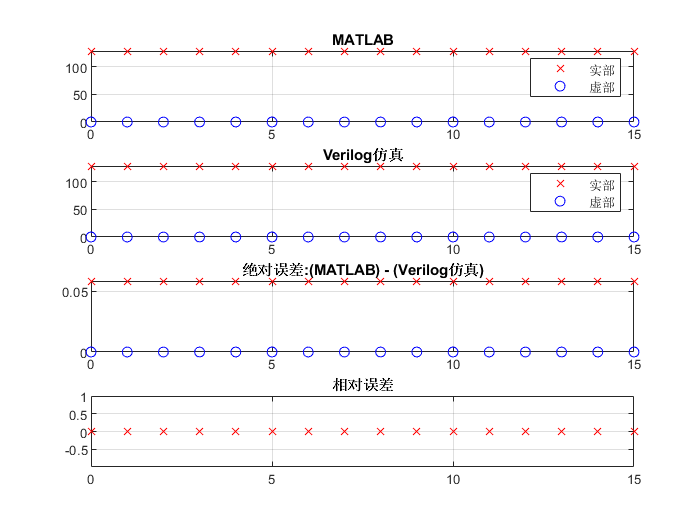
\includegraphics[width=0.45\linewidth]{Figure/result_i.png}}
        \subcaptionbox{数据2}{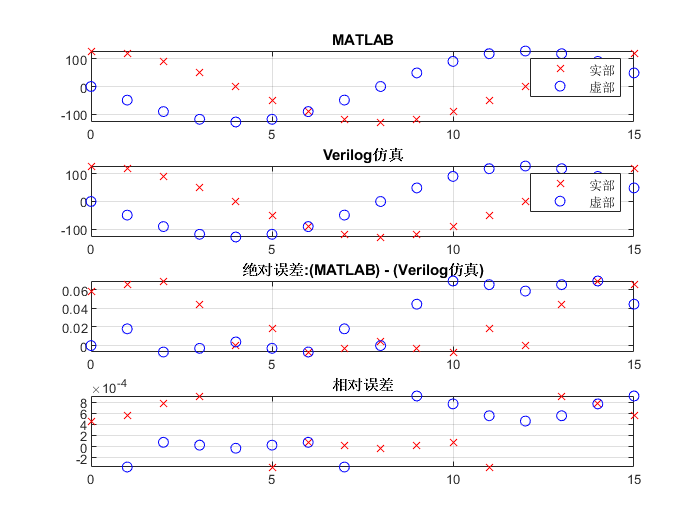
\includegraphics[width=0.45\linewidth]{Figure/result_ii.png}}\\
        \subcaptionbox{数据3}{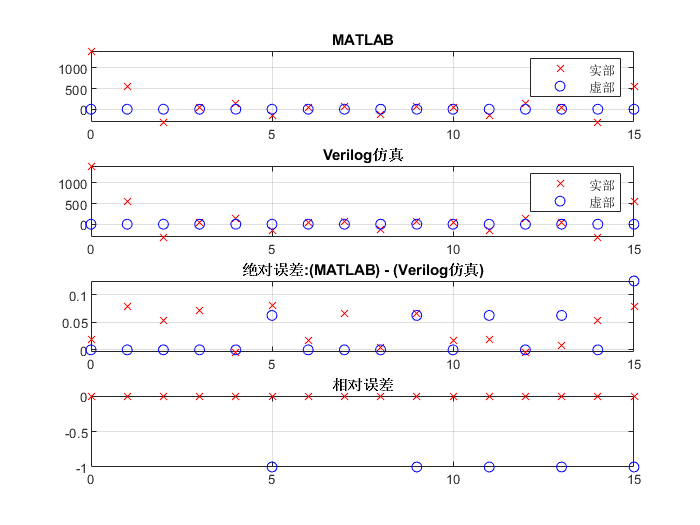
\includegraphics[width=0.45\linewidth]{Figure/result_iii.png}}
        \subcaptionbox{数据4}{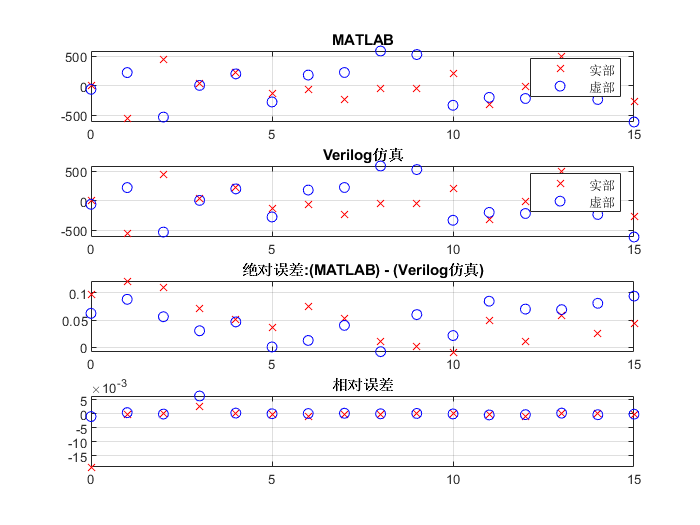
\includegraphics[width=0.45\linewidth]{Figure/result_iv.png}}
    \end{center}%
    \centering
\caption{数据对比}
    \label{fig:duibi}
\end{figure}

从图\ref{fig:duibi}可以发现,数据1,2,4绝对误差在0.05以内,相对误差在0.005以内,这些都是在容许的范围内。
数据3的绝对误差也在0.05以内,5,9,11,13处的相对误差为1原因可能是该点处的理论值较小,
造成了相对误差的扩大。

\chapter{总结}

本文分析了DIT-FFT的各个细节,从而用硬件描述语言实现了各个模块的编码。测试各个
模块正确之后,进行整体的算法设计。

最后,对整个设计进行实现、仿真、验证,并将计算结果与matlab计算结果进行
比较,观察FFT变换之后的仿真结果,通过数据分析得出本次设计的仿真结果与
matlab计算结果在允许的误差范围内完全吻合,达到设计要求。本设计虽然取得了
一些成果,但也存在一些不足:
\begin{enumerate}
    \item 本实验虽然采用了DIT-FFT的思路,但因为整个模块共用一定蝶形
        运算单元,因此运算速度必然会降低很多,同时,本实现没有优化具体
        的设计,换而言之,程序有优化的空间,使得运算速度加快。
    \item 本设计采用的是整数处理的方法,误差必然存在,对运算结果有一定的
        影响。
    \item 数据的输入和运算输出均采用串行传输,对于 $2^M$较大时,会产生
        很严重的时延,因此本程序不能直接扩展为高点数的FFT
\end{enumerate}

通过这次设计,我熟悉了FPGA先进期间和一些良好的设计思想和设计方法。
同时也提高了自己分析和解决问题的能力。这些都成为我以后学习工作中的参考。

